\documentclass[11pt]{article}
\usepackage[paper=letterpaper,margin=1in]{geometry}
\usepackage{graphics}
\usepackage{epsfig}
\usepackage{arcs}
\usepackage{fontenc}
\usepackage{alltt}
\usepackage{amssymb,amsfonts,epsf,url}
\usepackage{graphicx}
\usepackage{pstricks,pstricks-add}
\usepackage{pst-node}
\usepackage{pst-coil}
\usepackage{amsmath}
\usepackage{amsthm}
\usepackage{verbatim}

 \usepackage{graphicx}
\usepackage{pstricks,pstricks-add,xcolor}
\usepackage{pst-node}
\usepackage{pst-coil}
\usepackage{tikz}
\newtheorem{theorem}{Theorem}[section]
\newtheorem{lemma}[theorem]{Lemma}
\newtheorem{corollary}[theorem]{Corollary}
\newtheorem{proposition}[theorem]{Proposition}
\newtheorem{observation}{Observation}
\newtheorem{case}[theorem]{Case}
\newtheorem{subcase}[theorem]{SubCase}
\newtheorem{transrule}[theorem]{TransRule}
\newtheorem{branchrule}[theorem]{BranchRule}
\newtheorem{remark}[theorem]{Remark}
\newtheorem{assumption}[theorem]{Assumption}
\newtheorem{definition}[theorem]{Definition}
\newtheorem{fact}[theorem]{Fact}
\newtheorem{reduction}{Reduction Rules}[section]
\renewcommand{\labelenumi}{\arabic{enumi}.}
\renewcommand{\labelenumii}{\arabic{enumi}.\arabic{enumii}.}
\renewcommand{\labelenumiii}{\arabic{enumi}.\arabic{enumii}.\arabic{enumiii}.}
\renewcommand{\labelenumiv}{\arabic{enumi}.\arabic{enumii}.\arabic{enumiii}.\arabic{enumiv}.}
\newlength{\alginputwidth}
\newlength{\algboxwidth}
\newcommand{\alginput}[1]{\makebox[1.5cm][l]{ {\sc Input:}} \parbox[t]{\alginputwidth}{{\it #1}}}
\newcommand{\algoutput}[1]{\makebox[1.5cm][l]{ {\sc Output:}} \parbox[t]{\alginputwidth}{{\it #1}}}
\newcommand{\algtitle}[1]{\underline{Algorithm \ {\bf #1}} \vspace*{1mm}\\}

\newsavebox{\algbox}
\newsavebox{\captionbox}
\newenvironment{algorthm}[2]%
    {
        \setlength{\algboxwidth}{\columnwidth}
        \addtolength{\algboxwidth}{-\columnsep}
        \addtolength{\algboxwidth}{-1mm}
        \setlength{\alginputwidth}{\algboxwidth}
        \addtolength{\alginputwidth}{-1.7cm}
        \begin{figure}[tb]
            \vspace*{2mm}
            \centering
            \begin{lrbox}{\captionbox}
                \begin{minipage}[b]{\algboxwidth}
                    \centering
                    \caption{#1}
                    \label{#2}
                \end{minipage}
            \end{lrbox}
            \begin{lrbox}{\algbox}
                \begin{minipage}[b]{\algboxwidth}
                    \footnotesize
                    \vspace*{2mm}
    } % end of begin
    {
                    \vspace*{0.2mm}
               \end{minipage}
            \end{lrbox}
            \fbox{\usebox{\algbox}\hspace*{1mm}}
            \usebox{\captionbox}
            \vspace*{-4mm}
        \end{figure}
    }
\newsavebox{\algcodebox}
\newenvironment{codeblock}%
    {
        \begin{enumerate}
            \setlength{\itemsep}{2pt}
            \setlength{\parsep}{0pt}
            \setlength{\topsep}{0pt}
            \setlength{\parskip}{0pt}
            \setlength{\partopsep}{0pt}
    } % end of begin
    {\end{enumerate}}
\newcommand{\step}{\item}
\newcommand{\paramproblem}[4]{\noindent {\sc #1}
\\
{\bf Given:} #2\\
{\bf Parameter:} #3\\
{\bf Question:} #4}


\newcommand{\YES}{\textup{\textsf{YES}}}
\newcommand{\NO}{\textup{\textsf{NO}}}
\newcommand{\Oh}{{\mathcal O}}
\newcommand{\nat}{\mathbb{N}}

\newcommand{\Pol}{\mbox{$\mathcal P$}}
\newcommand{\NP}{\mbox{$\mathcal{NP}$}}

\def\eg{{\em e.g.}}
\def\cf{{\em cf.}}
\def\ie{{\em i.e.}}
\def\etal{{\em et al.}}



\psset{unit=1pt}

\date{16 March 2017}
\title{Put your title here}

\author{{\sc Nathaniel Brengle}\thanks{Address of Author 1. Email: {\tt nathaniel.brengle@gmail.com}}}


\begin{document}

\maketitle

\begin{abstract}
Summarize your work in 1-2 paragraphs.

\end{abstract}

\pagenumbering{roman}
\pagenumbering{arabic}


\section{Introduction} \label{sec:intro}
Introduce the problem(s) you study.

\subsection{Motivation and related work}
\label{subsec:motive}
Motivate your work, and review the related work in the literature.

\subsection{Results and techniques}
\label{subsec:results}
Summarize your results and techniques.

\section{Preliminaries}
\label{sec:prelim}
Introduce the terminologies you use, and review the necessary background.

\section{Section 1}
\label{subsec:structural}
The body of your paper should be structured in sections, where the material in each section has a common theme. For example, if your paper studies different aspects of a problem (\eg, complexity/\NP-hardness, approximation, exact algorithms), then the results pertaining to each aspect can be discussed under a separate section. Also, if you obtain structural results, or develop techniques, that are later used in different parts of the paper, then you may want to put them in a separate section (section 1) at the beginning of your paper.


We prove the following:

\begin{theorem}
$\Pol \neq \NP$.
\end{theorem}

\begin{proof}

\end{proof}

\begin{algorthm}{An algorithm to print out ``Hello World'' indefinitely.}{alg:hello}
\algtitle{``Hello World''}


\begin{codeblock}
\step Output ``Hello World'';

\step Go to step 1;

\end{codeblock}
\end{algorthm}




\begin{figure}[htbp]\label{fig:admissible}
\begin{center}
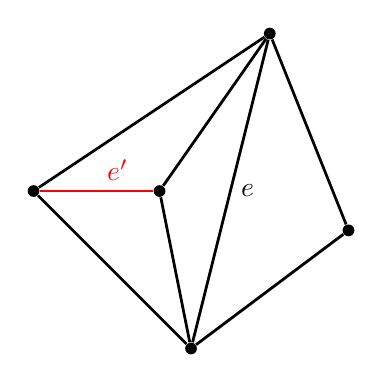
\begin{tikzpicture}
[vertex/.style={fill,circle,inner sep = 1.5pt}]

\node (x) at (7, 1) [vertex]{};
\node (a) at (4,-1) [vertex] {};
\node (b) at (5.6,-1) [vertex]{};
\node (c) at (8,-1.5) [vertex] {};
\node (d) at (6,-3) [vertex] {};


\draw[line width=1] (a) -- (x) -- (c) -- (d) -- (a);

\draw[black, line width=1] (x) -- (d) node[midway, anchor=west] {$e$};
\draw[black, line width=1] (x) -- (b) ;
\draw[black, line width=1] (b) -- (d) ;
\draw[red, line width=1] (b) -- (a) node[midway, anchor=south west] {$e'$};
\end{tikzpicture}

\end{center}
\caption{Illustration of ....}
\end{figure}



\section{Concluding remarks}
\label{sec:conclusion}
Summarize in a short paragraph the work you did. Discuss what future work and open questions ensue from your work.

\bibliographystyle{plain}
\bibliography{ref}
See the format of the attached bibliography file for referencing~\cite{ref1}.


\end{document}
